\documentclass[xcolor=table]{beamer}
\usepackage[utf8]{inputenc}
\usepackage[T1]{fontenc}
\usepackage[alf]{abntex2cite}
\usepackage{udesc}
\usepackage{amsfonts,amsmath,amssymb,mathtools}
\usepackage{verbatim}
\usepackage{listings}
\usepackage[ddmmyyyy]{datetime}
\usepackage{hyperref, url}
% \usepackage{titlepic}
\usepackage{graphicx}
\usepackage{bussproofs}
\usepackage{multirow}
\usepackage{changepage}
\usepackage{xspace}

\newcommand{\uglyphi}{\phi} % mantendo o \phi velho
\renewcommand \phi{\varphi}

\newcommand{\SisT}{\(\textbf{KT} \mathbin{\odot} \textbf{K4}\)\xspace}

\let \emptyset \varnothing
\newcommand{\miguel}[1]{\textcolor{violet}{\textbf{MIGUEL:} #1}}

\graphicspath{{Figuras/}}
\setbeamertemplate{frametitle continuation}{}

% suprimindo warnings do hyperref
\pdfstringdefDisableCommands{%
  \def\\{}%
  \def\texttt#1{#1}%
  \def\smallskip{}%
  \def\medskip{}%
}

\renewcommand{\figurename}{Figura}
\sloppy
\title[]{Implementação de uma biblioteca da Lógica de Inconsistência Formal LFI1 em Coq}

\author[Helena Vargas Tannuri]{
    Helena Vargas Tannuri\\\smallskip
    {\scriptsize Universidade do Estado de Santa Catarina \\\smallskip
    \vspace{-2mm}
    \texttt{helenavargastannuri@gmail.com}\\\medskip
    {Orientadora: Dra Karina Girardi Roggia}\\
    {Coorientador: Miguel Alfredo Nunes}
    }
}

\date[]{\today}

\begin{document}

    \begin{frame}
        \titlepage
    \end{frame}

    \begin{frame}[allowframebreaks]{Sumário}
        \tableofcontents
    \end{frame}

    \section[]{Introdução}
    \begin{frame}{Introdução}
        \begin{itemize}
            \item Lógicas paraconsistentes são sistemas não-clássicos que separam a trivialidade da contradição;
            \begin{itemize}
                \item[--] Usualmente, lógicas ortodoxas assumem que toda teoria contraditória é uma teoria trivial, ou seja, uma teoria com todas as fórmulas.
            \end{itemize}
            \item Lógica não-clássica é qualquer lógica que quebra algum dos princípios da lógica clássica;
            \begin{itemize}
                \item[--] As lógicas paraconsistentes quebram o princípio da explosão (definido como $\alpha \to (\neg \alpha \to \beta)$)~\cite{carnielli2007}.
            \end{itemize}
            \item Lógicas de inconsistência formal (\textbf{LFI}s) são lógicas paraconsistentes que resgatam de maneira \textit{controlada} o princípio da explosão, internalizando o conceito de inconsistência dentro da sua linguagem~\cite{Carnielli_Coniglio_2016}.
        \end{itemize}
    \end{frame}

    \begin{frame}{Introdução}
        \begin{itemize}
            \item Lógicas paraconsistentes possuem diversas aplicações em diferentes campos do conhecimento;
        \end{itemize}
    \end{frame}

    \begin{frame}{Introdução}
        \begin{itemize}
            \item Assistentes de provas são softwares para desenvolvimento de provas formais;
            \item Coq é um assistente de provas com grande disponibilidade de materiais didáticos e diversas ferramentas que facilitam no desenvolvimento de provas~\cite{silva2019certificacao};
            \item Fusões de lógicas é um tópico complexo, porém as dificuldades referentes a isso podem ser amenizadas com o uso de assistentes de provas como o Coq.
            \item Continuação do que foi desenvolvido em~\cite{silveira2020implementacao} e~\cite{silveira2022sound}.
        \end{itemize}
    \end{frame}

    \section[]{Objetivos}
    \begin{frame}{Objetivo Geral}
        Modelar, no assistente Coq, sistemas de lógicas multimodais resultantes da fusão de lógicas modais mais simples,
		preservando propriedades das lógicas combinadas.
    \end{frame}

    \begin{frame}{Objetivos Específicos}
        \begin{enumerate}
			\item Estudar os principais conceitos de combinações de lógicas, em especial, a fusão;
			\item Realizar um estudo de caso de fusões de lógicas modais no Coq;
			\item Modelar, de forma paramétrica, sistemas de lógicas multimodais resultantes de fusão de lógicas modais em Coq.
		\end{enumerate}
    \end{frame}

    \section[]{Trabalhos Relacionados}
    \begin{frame}{Trabalhos Relacionados}
        \begin{enumerate}
            \item \citeauthoronline{benzmuller2010combining} (\citeyear{benzmuller2010combining}) -
                apresenta fusões de lógicas modais em Cálculo-\(\lambda\) Simplesmente Tipado e modelagem de lógicas combinadas em diversos assistentes de provas;
            \item \citeauthoronline{fuenmayor2019mechanised} (\citeyear{fuenmayor2019mechanised}) -
                descrevem lógicas modais resultantes de combinação em Isabelle;
            \item \citeauthoronline{lescanne2007dynamic} (\citeyear{lescanne2007dynamic}) -
                descrevem uma lógica modal resultante de fusão em Coq;
            \item \citeauthoronline{rabe2017identify} (\citeyear{rabe2017identify}) -
                modela sistemas lógicos e combinações de lógicas em uma linguagem baseada em teoria de tipos chamada M\textsubscript{MT}.
        \end{enumerate}
    \end{frame}

    \section[]{Lógica Modal}
    % \begin{frame}{Lógica Modal}
    %     \begin{itemize}
    %         \item Diversos tipos de lógicas modais - interpretações diferentes para modalidades;
    %         \item Lógica modal alética contém duas modalidades \(\Box\) e \(\Diamond\) indicam necessidade e possibilidade;
    %         \item Lógica temporal - formalismo para verificação de programas, ~\cite{pnueli1977temporal} foi o primeiro,
    %         \citeauthoronline{lamport2002specifying} e TLA+ recentemente.
    %     \end{itemize}
    % \end{frame}

    \begin{frame}{Lógica Modal - Linguagem}
        Menor conjunto \textsf{LM} que respeita:

        \vspace{\baselineskip}

        \begin{enumerate}
            \item \(\top, \bot \in \mathsf{LM} \)
            \item \(\mathbb{P} \subseteq \mathsf{LM}\)
            \item \(\text{Se } \phi \in \mathsf{LM} \text{, então } \circ \phi \in \mathsf{LM}, \text{ sendo } \circ \in \{\Box, \Diamond, \neg\}\)
            \item \(\text{Se } \phi, \psi \in \mathsf{LM} \text{, então } \phi \circ \psi \in \mathsf{LM}, \text{ sendo } \circ \in \{\land, \lor, \to\}\)
        \end{enumerate}
    \end{frame}

    \begin{frame}{Lógica Modal - Semântica}
        \begin{block}{Frames}
            Um frame é um par \(\mathcal{F} = \langle \mathcal{W}, \mathcal{R} \rangle\), onde \(\mathcal{W} \neq \emptyset\) e
            \(\mathcal{R} \subseteq \mathcal{W} \times \mathcal{W}\).
        \end{block}

        \vspace{2\baselineskip}

        \begin{block}{Modelos}
            Modelos são pares de frames e funções de valoração da forma
            \({\mathcal{M} = \langle \mathcal{F}, \mathcal{V} \rangle}\), onde \(\mathcal{V}\) é uma função total binária
            definida por \(\mathcal{V}: \mathbb{P} \to 2^{\mathcal{W}}\)
        \end{block}
    \end{frame}

    % \begin{frame}{Lógica Modal - Semântica}
    %     \begin{align*}
    %         \mathcal{M}, w_0 & \Vdash \top  \\
    %         \mathcal{M}, w_0 & \nVdash \bot \\
    %         \mathcal{M}, w_0 & \Vdash p_i \text{ sse } w_0 \in \mathcal{V}(p_i), \text{ para } p_i \in \mathbb{P} \\
    %         \mathcal{M}, w_0 & \Vdash \neg \phi \text{ sse } \mathcal{M}, w_0 \nVdash \phi \\
    %         \mathcal{M}, w_0 & \Vdash \phi \land \psi \text{ sse } (\mathcal{M}, w_0 \Vdash \phi \text{ e } \mathcal{M}, w_0 \Vdash \psi) \\
    %         \mathcal{M}, w_0 & \Vdash \phi \lor \psi \text{ sse } (\mathcal{M}, w_0 \Vdash \phi \text{ ou } \mathcal{M}, w_0 \Vdash \psi) \\
    %         \mathcal{M}, w_0 & \Vdash \phi \to \psi \text{ sse } (\mathcal{M}, w_0 \nVdash \phi \text{ ou } \mathcal{M}, w_0 \Vdash \psi) \\
    %         \mathcal{M}, w_0 & \Vdash \Box \phi \text{ sse } \forall w_1 \in \mathcal{W}, (w_0 \mathcal{R} w_1 \to
    %                          \mathcal{M}, w_1 \Vdash \phi ) \\
    %         \mathcal{M}, w_0 & \Vdash \Diamond \phi \text{ sse } \exists w_1 \in \mathcal{W}, (w_0 \mathcal{R} w_1 \land
    %                          \mathcal{M}, w_1 \Vdash \phi )
    %     \end{align*}
    % \end{frame}

    \begin{frame}{Lógica Modal - Sintaxe}
        Axiomatização de Hilbert, 10 axiomas proposicionais:
        \begin{align*}
            &p_0 \to (p_1 \to p_0) \tag{Ax1} \\
            &(p_0 \to (p_1 \to p_2)) \to ((p_0 \to p_1) \to (p_0 \to p_2)) \tag{Ax2} \\
            &(\neg p_1 \to \neg p_0) \to (p_0 \to p_1) \tag{Ax3} \\
            &p_0 \to (p_1 \to (p_0 \land p_1)) \tag{Ax4} \\
            &(p_0 \land p_1) \to p_0 \tag{Ax5} \\
            &(p_0 \land p_1) \to p_1 \tag{Ax6} \\
            &p_0 \to (p_0 \lor p_1) \tag{Ax7} \\
            &p_1 \to (p_0 \lor p_1) \tag{Ax8} \\
            &(p_0 \to p_2) \to ((p_1 \to p_2) \to (p_0 \lor p_1) \to p_2) \tag{Ax9} \\
            &\neg \neg p_0 \to p_0 \tag{Ax10}
        \end{align*}
    \end{frame}

    \begin{frame}{Lógica Modal - Axiomas Modais e Regras de Derivação}
        Axiomatização de Hilbert, 2 axiomas modais:
        \begin{align*}
            &\Box (p_0 \to p_1) \to (\Box p_0 \to \Box p_1) \tag{K}\\
            &\Diamond (p_0 \lor p_1) \to (\Diamond p_0 \lor \Diamond p_1) \tag{Possibilidade}
        \end{align*}

        E regras de Necessitação e Modus Ponens:

        \vspace{\baselineskip}

        \begin{minipage}{.45\textwidth}
            \begin{prooftree}
                \AxiomC{$\Gamma \vdash \phi$}
                \RightLabel{Nec}
                \UnaryInfC{$\Gamma \vdash \Box \phi$}
            \end{prooftree}
        \end{minipage}%
        \begin{minipage}{.45\textwidth}
            \begin{prooftree}
                \AxiomC{$\Gamma \vdash \phi \to \psi$}
                \AxiomC{$\Gamma \vdash \phi$}
                \RightLabel{MP}
                \BinaryInfC{$\Gamma \vdash \psi$}
            \end{prooftree}
        \end{minipage}
    \end{frame}

    \begin{frame}{Lógica Modal - Metapropriedades}
        % \miguel{Conferir para casos da completude/corretude fortes}
        % \begin{block}{Corretude Fraca}
        %     Se há uma derivação sintática para uma fórmula, então há uma derivação semântica em algum frame/modelo:
        %     \(\vdash \phi \Rightarrow \ \vDash \phi\)
        % \end{block}

        \begin{block}{Corretude Forte}
            Se há uma derivação sintática para uma fórmula a partir de uma teoria, então há uma derivação semântica em algum frame/modelo a partir da mesma teoria:
            \(\Gamma \vdash \phi \Rightarrow \ \Gamma \vDash \phi\)
        \end{block}

        \vspace{2\baselineskip}

        % \begin{block}{Completude Fraca}
        %     Se há uma derivação semântica para uma fórmula em algum frame/modelo, então há uma derivação sintática:
        %     \(\vDash \phi \Rightarrow \ \vdash \phi\)
        % \end{block}

        \begin{block}{Completude Forte}
            Se há uma derivação semântica para uma fórmula em algum frame/modelo a partir de uma teoria, então há uma derivação sintática a partir da mesma teoria:
            \(\Gamma \vDash \phi \Rightarrow \ \Gamma \vdash \phi\)
        \end{block}
    \end{frame}

    \subsection[]{Lógicas Multimodais}
    \begin{frame}{Lógicas Multimodais}
        Extensão do conceito de lógica modais com apenas uma (ou um par de) modalidade(s) que contém diversas modalidades.
        A linguagem de uma lógica multimodal é o menor conjunto \(\mathsf{LM}_n\) que respeita:

        \vspace{\baselineskip}

        \begin{enumerate}
            \item \(\top, \bot \in \mathsf{LM}_n \)
            \item \(\mathbb{P} \subseteq \mathsf{LM}_n\)
            \item \(\text{Se } \phi \in \mathsf{LM}_n \text{, então } \circ \phi \in \mathsf{LM}_n, \text{ sendo } \circ \in \{\Box_1, \dots, \Box_n, \Diamond_1, \dots, \Diamond_n, \neg\}\)
            \item \(\text{Se } \phi, \psi \in \mathsf{LM}_n \text{, então } \phi \circ \psi \in \mathsf{LM}_n, \text{ sendo } \circ \in \{\land, \lor, \to\}\)
        \end{enumerate}

        % \vspace{\baselineskip}

        % % São adicionados novas instâncias dos axiomas (K) e (Possibilidade), uma para cada \(\Box_i \text{ e }\Diamond_i\).
    \end{frame}

    \begin{frame}{Lógicas Multimodais}
        \begin{block}{n-frames}
            Um n-frame é uma tupla \({\mathcal{F}_n = \langle \mathcal{W}, \mathcal{R}_1,\dots,\mathcal{R}_n \rangle}\), onde \(\mathcal{W} \neq \emptyset\) e
            \(\mathcal{R}_i \subseteq \mathcal{W} \times \mathcal{W}, 1 \leq i \leq n\).
        \end{block}

        \vspace{\baselineskip}

        Para cada \(\Box_i/\Diamond_i\) tem-se:
        \begin{align*}
            &\Box_i (p_0 \to p_1) \to (\Box_i p_0 \to \Box_i p_1)\\
            &\Diamond_i (p_0 \lor p_1) \to (\Diamond_i p_0 \lor \Diamond_i p_1)
        \end{align*}

        Regra de Necessitação é substituída por:

        \begin{prooftree}
            \AxiomC{$\Gamma \vdash \phi$}
            \RightLabel{\(\textnormal{Nec}_i\)}
            \UnaryInfC{$\Gamma \vdash \Box_i \phi$}
        \end{prooftree}
    \end{frame}

    \section[]{Fusão de Lógicas Modais}
    \begin{frame}{Fusão de Lógicas Modais}
        \begin{itemize}
            \item Método para combinar sistemas lógicos distintos original desenvolvido por~\cite{thomason1984combinations};
            \item Possibilita especificar sistemas lógicos com múltiplas modalidades distintas, dados dois sistemas lógicos mais simples;
            \item A fusão de lógicas preserva corretude e completude - sendo \(\mathcal{L}_1\) e \(\mathcal{L}_2\) lógicas corretas/completas
                    uma lógica \(\mathcal{L}_3\) resultante da sua fusão também será correta/completa;
            \item Preservação de corretude e completude foi originalmente demonstrada por~\cite{fine1996transfer}, prova se resume a construir
                    modelos para \(\mathcal{L}_{3}\) a partir de certos modelos para \(\mathcal{L}_1\) e \(\mathcal{L}_2\).
        \end{itemize}
    \end{frame}

    \begin{frame}{Fusão de Lógicas Modais}
        \begin{itemize}
            \item Sendo \(\mathcal{L}_1\) e \(\mathcal{L}_2\) lógicas modais:
                \begin{itemize}
                    \item[--] Linguagens são \(\mathsf{LM}_1\) e \(\mathsf{LM}_2\);
                    \item[--] Correspondentes as classes \(\mathfrak{F}_{1}\) e \(\mathfrak{F}_{2}\)
                    \item[--] Axiomatizadas pelos conjuntos de axiomas \(\Sigma_1\) e \(\Sigma_2\) com regras \(Nec_1\) e \(Nec_2\) respectivamente.
                \end{itemize}
            \item A lógica \(\mathcal{L}_{3} = \mathcal{L}_1 \mathbin{\odot} \mathcal{L}_2\):
            \begin{itemize}
                \item[--] Terá linguagem \(\mathsf{LM}_{3} = \mathsf{LM}_{1} \cup \mathsf{LM}_{2}\);
                \item[--] Será correspondente à classe \(\mathfrak{F}_{3}\) de 2-frames da forma \(\langle \mathcal{W}, \mathcal{R}, \mathcal{S}\rangle\),
                        onde \(\langle \mathcal{W}, \mathcal{R}\rangle \in \mathfrak{F}_{1}\) e \(\langle \mathcal{W}, \mathcal{S}\rangle \in \mathfrak{F}_{2}\)
                \item[--] Será axiomatizada por \(\Sigma_3 = \Sigma_1 \oplus \Sigma_2\) com regras \(Nec_1\) e \(Nec_2\).
            \end{itemize}
        \end{itemize}
    \end{frame}

    \section[]{Coq}
    \begin{frame}{Coq}
        \begin{itemize}
            \item Assistente de provas para lógica de alta ordem, capaz de descrever e raciocinar sobre objetos matemáticos~\cite{geuvers2009proof};
            \item O Coq é baseado em teoria de tipos, devido a Correspondência de Curry-Howard é capaz de expressar sistemas lógicos sofisticados;
            \item Coq tem uma grande quantidade de ferramentas de automação de provas, e também permite que seus usuários desenvolvam suas próprias ferramentas;
            \item Essas características tornam Coq uma boa ferramenta para representar sistemas lógicos complexos e operar sobre eles.
        \end{itemize}
    \end{frame}

    \section[]{Implementação}
    \begin{frame}{Implementação}
        \begin{itemize}
            \item A biblioteca de lógica modal desenvolvida em~\cite{silveira2020implementacao} e~\cite{silveira2022sound} serviu de base para a implementação;
            \item Foi provada a corretude do sistema \SisT;
            \item Foi modelada, de forma paramétrica, a fusão de sistemas sintáticos de lógicas modais;
            \item Foi modelada a semântica de sistemas multimodais.
        \end{itemize}
    \end{frame}

    \begin{frame}{Implementação}
        \begin{figure}[htbp]
            \centering
            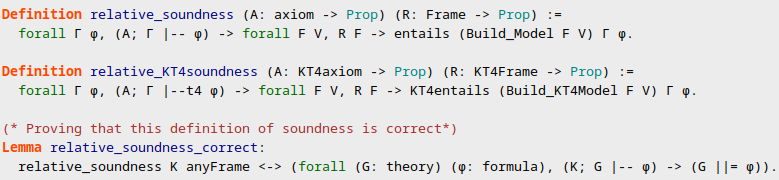
\includegraphics[width=\linewidth+.7cm,keepaspectratio]{KT4RelativeSoundness.png}
            \begin{flushleft}
                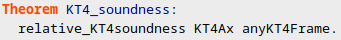
\includegraphics[scale=.6]{KT4Soundness.png}
            \end{flushleft}
            \caption{Corretude de \SisT}
        \end{figure}
    \end{frame}

    \begin{frame}{Implementação}
        \begin{figure}[htbp]
            \centering
            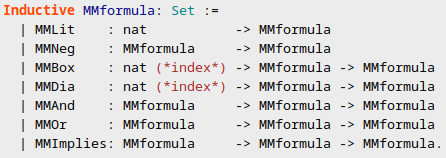
\includegraphics[scale=.6]{LinguagemMM.png}
            \caption{Linguagem do Sistema Multimodal}
        \end{figure}
    \end{frame}

    \begin{frame}{Implementação}
        \begin{figure}[htbp]
            \centering
            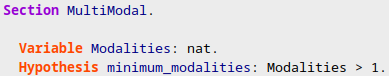
\includegraphics[scale=.6]{VariavelModalidades.png}
            \caption{Definição da Variável do Número de Modalidades no Sistema}
        \end{figure}
    \end{frame}

    \begin{frame}{Implementação}
        \begin{adjustwidth}{-.8cm}{}
            \begin{figure}[htbp]
                \centering
                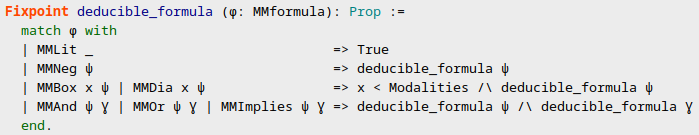
\includegraphics[scale=.5]{FormulaDedutivel.png}
                \begin{flushleft}
                    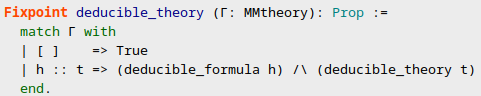
\includegraphics[scale=.5]{TeoriaDedutivel.png}
                \end{flushleft}
                \caption{Definição de Dedutibilidade de Fórmulas e Teorias}
            \end{figure}
        \end{adjustwidth}
    \end{frame}

    \begin{frame}{Implementação}
        \begin{figure}[htbp]
            \centering
            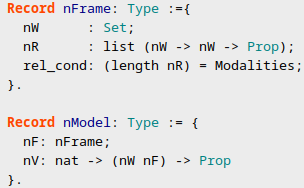
\includegraphics[scale=.6]{FramesModelosMM.png}
            \caption{Frames e Modelos Multimodais}
        \end{figure}
    \end{frame}

    \begin{frame}{Implementação}
        \begin{figure}[htbp]
            \centering
            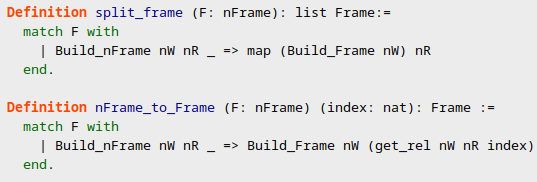
\includegraphics[scale=.6]{FrameMM->Frame.png}
            \caption{Função de Tradução de Frames Multimodais para Frames Monomodais}
        \end{figure}
    \end{frame}

    \begin{frame}{Implementação}
        \begin{adjustwidth}{-.5cm}{}
            \begin{figure}[htbp]
                \centering
                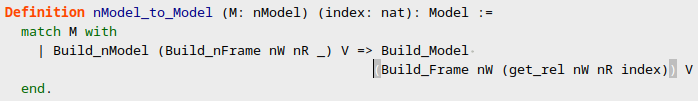
\includegraphics[scale=.475]{ModeloMM->Modelo}
                \caption{Função de Tradução de Modelos Multimodais para Modelos Monomodais}
            \end{figure}
        \end{adjustwidth}
    \end{frame}

    \begin{frame}{Implementação}
        \begin{adjustwidth}{-.5cm}{}
            \begin{figure}[htbp]
                \centering
                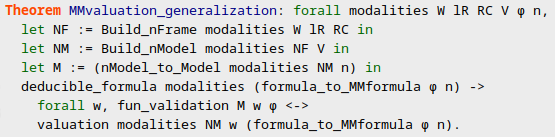
\includegraphics[scale=.6]{ProvaGeneralizacaoValoracao.png}
                \caption{Extensão da Valoração}
            \end{figure}
        \end{adjustwidth}
    \end{frame}

    \begin{frame}{Implementação}
        \begin{adjustwidth}{-1cm}{}
            \begin{figure}[htbp]
                \centering
                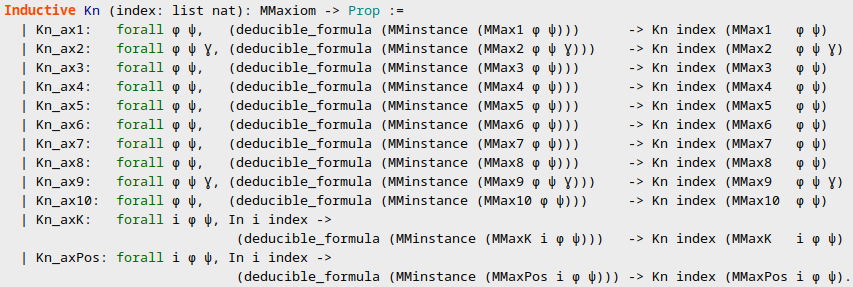
\includegraphics[scale=.425]{SistemaKMM.png}
                \caption{Axiomatização Multimodal do Sistema K}
            \end{figure}
        \end{adjustwidth}
    \end{frame}

    \begin{frame}{Implementação}
        \begin{adjustwidth}{-.5cm}{}
            \begin{figure}[htbp]
                \centering
                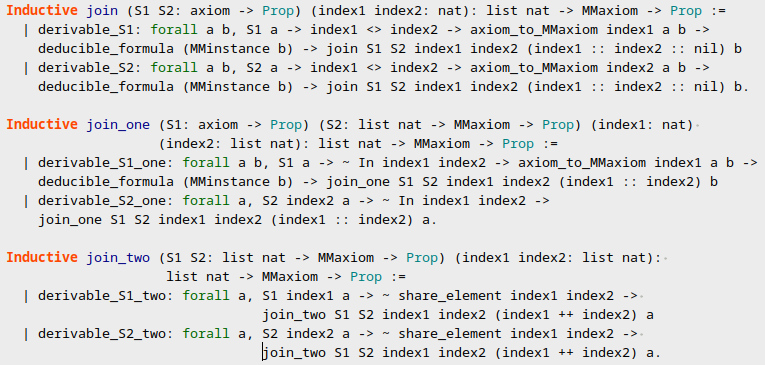
\includegraphics[scale=.45]{FusaoSistemasSintaticos.png}
                \caption{Definição de Fusão de Sistemas Sintáticos}
            \end{figure}
        \end{adjustwidth}
    \end{frame}

    \begin{frame}{Implementação}
        \begin{adjustwidth}{-.9cm}{}
            \begin{figure}[htbp]
                \centering
                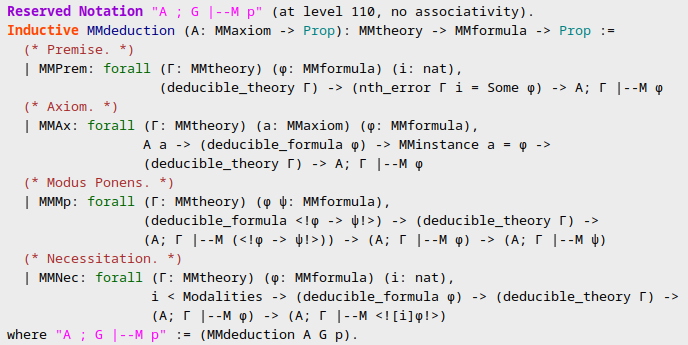
\includegraphics[scale=.5]{SistemaHilbert.png}
                \caption{Regras de Derivação do Sistema de Hilbert}
            \end{figure}
        \end{adjustwidth}
    \end{frame}

    \begin{frame}{Implementação}
        \begin{adjustwidth}{-.7cm}{}
            \begin{figure}[htbp]
                \centering
                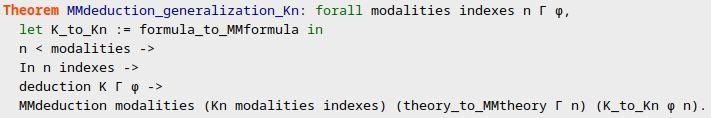
\includegraphics[scale=.5]{ProvaGeneralizacaoDerivacaoKMM.png}
                \caption{Prova de Generalização da Dedução para K\textsubscript{n}}
            \end{figure}
        \end{adjustwidth}
    \end{frame}

    \begin{frame}{Implementação}
        \begin{adjustwidth}{0cm}{}
            \begin{figure}[htbp]
                \centering
                \begin{flushleft}
                    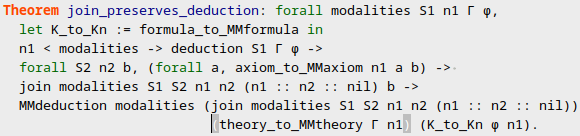
\includegraphics[scale=.5]{Figuras/ProvaJoinPreservaDeducao.png}
                    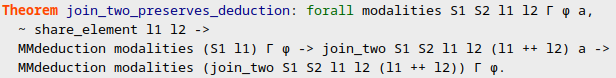
\includegraphics[scale=.5]{Figuras/ProvaJoinTwoPreservaDeducao.png}
                \end{flushleft}
                \caption{Prova da Preservação de Deduções pela Fusão}
            \end{figure}
        \end{adjustwidth}
    \end{frame}

    \begin{frame}{Implementação}
        \begin{adjustwidth}{0cm}{}
            \begin{figure}[htbp]
                \centering
                \begin{flushleft}
                    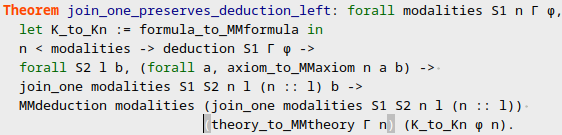
\includegraphics[scale=.5]{Figuras/ProvaJoinOnePreservaDeducao1.png}
                    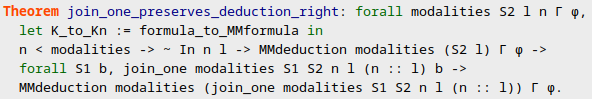
\includegraphics[scale=.5]{Figuras/ProvaJoinOnePreservaDeducao2.png}
                \end{flushleft}
                \caption{Prova da Preservação de Deduções pela Fusão}
            \end{figure}
        \end{adjustwidth}
    \end{frame}

    \begin{frame}{Dificuldades na Implementação}
        \begin{itemize}
            \item Representação da linguagem do sistema multimodal - Não representa união de linguagens;
            \item Definição de frames multimodais - Não foi possível representar fusão de frames e uso da função \texttt{nth};
            \item Tradução de modelos multimodais para modelos monomodais;
            \item Corretude do Sistema \SisT não foi provada pelo método de transferência.
        \end{itemize}
    \end{frame}

    \section[]{Conclusões}
    \begin{frame}{Conclusões}
        \begin{itemize}
            \item Uma implementação paramétrica de fusão de sistemas sintáticos semelhante a desenvolvida nesse trabalho não foi encontrado nos trabalhos relacionados;
            \item Não foi possível terminar a implementação da fusão de sistemas semânticos devido a escolhas de implementação da biblioteca base;
            \item Não foi possível demonstrar transferência de propriedades no Coq.%Demonstrar transferência de propriedades no Coq se mostrou estar além do escopo deste trabalho.
        \end{itemize}
    \end{frame}

    \section[]{Referências}
    \begin{frame}[allowframebreaks]{Referências}
        \bibliography{referencias}
    \end{frame}

\end{document}